\documentclass[__main__.tex]{subfiles}
\begin{document}

\qtitle{С}{03}
Закон Кулона, напряжённость поля, силовые линии электростатического поля, эквипотенциальные поверхности, электростатическая защита.\\

\textbf{Закон Кулона:} Для постоянного электрического поля уравнения Максвелла имеют вид:
$$
\begin{cases}
\operatorname{div}\vec{E} = 4 \pi \rho\\
\operatorname{rot}\vec{E} = 0\\
\end{cases}
$$
Абсолютная величина напряженности поля $E$ будет зависеть только от расстояния $R$ до заряда $e$. Для нахождения этой абсолютной величины применим уравнение
$$
    \operatorname{div}\vec{E}=4\pi\rho
$$
в интегральной форме
$$
    \oint\vec{E}df=4\pi\int\rho dV.
$$
Поток электрического поля через шаровую поверхность с радиусом $R$, проведенную вокруг заряда $e$, равен $4\pi R^2 E$; этот поток должен быть равен $4\pi e$. Тогда:
$$
    E=\frac{e}{R^2}
$$
В векторном виде:
$$
    \vec{E}=\frac{e \vec{R}}{R^3}
$$
Это и есть \textbf{закон Кулона} (Поле, создаваемое точечным зарядом, обратно пропорционально квадрату расстояния до этого заряда)
Напряженность поля. Силу первого рода, отнесенную к заряду, равному единице, называют \textbf{напряженностью электрического поля}:\\
$$
    \vec{E} = -\frac{1}{c}\frac{\partial \vec{A}}{\partial t}-\nabla\varphi,
$$
где $\vec{A}$ -- векторный потенциал поля. Для того чтобы описать электрическое поле, нужно задать вектор напряженности в каждой точке поля. Это можно сделать аналитически или графически. Для этого пользуются \textbf{силовыми линиями} -- это линии, касательная к которым в любой точке поля совпадает с направлением вектора напряженности $\vec{E}$:
\begin{figure}[h]
\centering
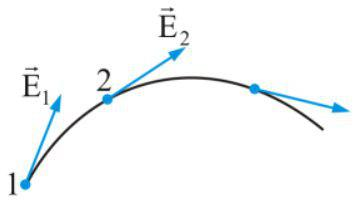
\includegraphics[width=.5\linewidth]{С-03_1.jpg}
\end{figure}
Для системы зарядов, как видим, силовые линии направлены от положительного заряда к отрицательному:
\begin{figure}[h]
\centering
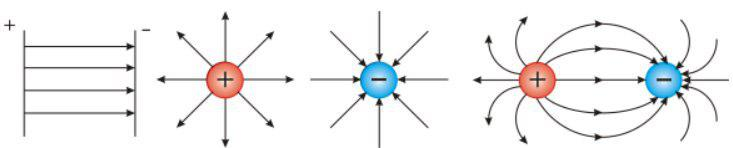
\includegraphics[width=.9\linewidth]{С-03_2.jpg}
\end{figure}
\textbf{Эквипотенциальные поверхности} -- это воображаемые поверхности все точки которой имеют одинаковый потенциал.
\begin{gather*}
    U(x,y,z) = const
\end{gather*}
\textbf{Электростатическая защита} -- защита приборов и оборудования, основанная на том, что напряженность электростатического поля внутри проводника равна нулю.\\
Потенциал электростатического поля:
$$
    \varphi=\frac{e}{R}
$$
Работа поля по перемещению заряда из одной точки в другую, называется разностью потенциалов.\\

\end{document}